\section{ナノサイエンス・デバイス}
\label{sec:ナノデバイス}

\subsection{分野の概要}
半導体材料や高分子材料など、20世紀の科学技術研究の中で生まれた物質群は、100種類ほどの元素の無限とも言える組み合わせの中から見出され、特異な機能や新しい現象の発現を通して、現代社会の産業基盤を形成してきた。これらの物質や材料をミクロな視点に立って研究する物質科学は、物性科学、分子科学、材料科学という三つの学問分野にまたがり、基礎研究と応用研究をつなぐ役割をも担う、広大な学問分野である。

半導体材料や高分子材料など、20世紀の科学技術研究の中で生まれた物質群は、100種類ほどの元素の無限とも言える組み合わせの中から見出され、特異な機能や新しい現象の発現を通して、現代社会の産業基盤を形成してきた。これらの物質や材料をミクロな視点に立って研究する物質科学は、物性科学、分子科学、材料科学という三つの学問分野にまたがり、基礎研究と応用研究をつなぐ役割をも担う、広大な学問分野である。

半導体材料や高分子材料など、20世紀の科学技術研究の中で生まれた物質群は、100種類ほどの元素の無限とも言える組み合わせの中から見出され、特異な機能や新しい現象の発現を通して、現代社会の産業基盤を形成してきた。これらの物質や材料をミクロな視点に立って研究する物質科学は、物性科学、分子科学、材料科学という三つの学問分野にまたがり、基礎研究と応用研究をつなぐ役割をも担う、広大な学問分野である。

\paragraph{}
コミュニティからの意見は、
物質科学分野では、討論会「エクサスケールコンピュータへの期待」(2012年7月13日、東大物性研)、日本物理学会計算物質科学インフォーマルミーティング(2012年9月18日、横国大)、TCCI研究会(2012年10月9日、分子研)、計算物質科学シンポジウム(2012年10月22日、東大物性研)、CMSI研究会(2012年12月3日、分子研)、日本化学会特別企画「超巨大計算時代の化学」(2013年3月25日、立命館大)、日本物理学会シンポジウム「エクサスケールに向けて歩み出す計算物理学」において、実験家、企業研究者も含めたコミュニティ全体に対しロードマップを紹介し、パネルディスカッションなどを通じて意見収集を行った。具体的には、J-PARC、SPring-8、SACLAといった大型実験施設との連携強化、元素戦略(磁石、触媒・電池、電子材料、構造材料分野)への計算物質科学からの貢献への期待などの意見を得ることができた。また、最先端HPCだけでなく、非専門家がPCあるいはクラスターワークステーションでシミュレーションを実行できるよう計算物質科学コミュニティ全体でアプリケーション・ソフトウェアを整備することや、莫大なシミュレーション結果や実験結果を保存・公開する仕組みを整備することなどに対する強い要望があった。

\paragraph{}
この分野における諸外国の動向は、
[ダミー原稿]、[ダミー原稿]、[ダミー原稿]、[ダミー原稿]、[ダミー原稿]、[ダミー原稿]、[ダミー原稿]、[ダミー原稿]、[ダミー原稿]。

\paragraph{}
各課題の概要は以下の通り。

\rmproject{次世代先端デバイス科学}
[ダミー原稿]、[ダミー原稿]、[ダミー原稿]、[ダミー原稿]、[ダミー原稿]、[ダミー原稿]、[ダミー原稿]、[ダミー原稿]、[ダミー原稿]。

\rmproject{分子機能と物質変換}
[ダミー原稿]、[ダミー原稿]、[ダミー原稿]、[ダミー原稿]、[ダミー原稿]、[ダミー原稿]、[ダミー原稿]、[ダミー原稿]、[ダミー原稿]。

\rmproject{エネルギー変換}
[ダミー原稿]、[ダミー原稿]、[ダミー原稿]、[ダミー原稿]、[ダミー原稿]、[ダミー原稿]、[ダミー原稿]、[ダミー原稿]、[ダミー原稿]。

\rmproject{マルチスケール材料科学}
[ダミー原稿]、[ダミー原稿]、[ダミー原稿]、[ダミー原稿]、[ダミー原稿]、[ダミー原稿]、[ダミー原稿]、[ダミー原稿]、[ダミー原稿]。

\rmproject{新量子相・新物質の基礎科学}
[ダミー原稿]、[ダミー原稿]、[ダミー原稿]、[ダミー原稿]、[ダミー原稿]、[ダミー原稿]、[ダミー原稿]、[ダミー原稿]、[ダミー原稿]。


\subsection{長期目標と社会貢献}
物性科学は$10^{23}$ほどの膨大な数の原子、分子多体系から成る自然を理解する営みを通じて、相転移にともなう自発的対称性の破れ、集団運動励起やトポロジー励起、マクロ量子現象といった基礎科学を一新する普遍概念をもたらし、素粒子物理学から経済学まで広がるさまざまな学問分野に大きな影響を与えてきた。

分子科学は、化学反応の理解とそれに基づく新しい分子・分子集合体の創製を通じて、物質科学研究に大きな展開をもたらしてきた。

材料科学は、一辺の長さが原子10個分くらいに相当するナノメートルのスケールで物質材料を捉えることにより、金属組織や粒界、複合材料など、材料としての利用に係る諸問題の解決を目指してきた。

これらの成果は、20世紀以降の産業・先端技術革新を生み出す基盤となった。トランジスタ、トンネルダイオード、半導体レーザー、集積回路、巨大磁気抵抗素子、CCD(電荷結合素子)、有機ELなどの革新デバイス、合成樹脂や導電性高分子などの新材料は、ノーベル賞の受賞対象ともなった物質科学の基礎研究が生んだ例である。
同じく物質科学の精華である超伝導は、最先端の医療用MRIの超伝導マグネットに使われ、更に超伝導リニアモーターやエネルギー損失のない電力線として実用化されようとしている。
高効率の太陽電池や高効率熱電素子など、地球規模のエネルギー問題解決に向けた新しい概念に基づくデバイスも、物質科学の基礎研究に基づいて提案され始めている。燃料電池に用いられる白金触媒、色素増感太陽電池に用いられるルテニウム、透明電極に使われるインジウム、リチウムイオン電池材料のリチウムやコバルトなど供給量が希少、あるいは今後の需要増に応じて希少になると考えられる元素の代替材料を他国に先駆けて開発することが、わが国の産業競争力を高めるためにも必要である。

一方、原子の組み合わせからさまざまな官能基・分子ができ、その多様な組み合わせで、溶液・ミセル・脂質膜・タンパク質・高分子・クラスレートハイドレートなどが形成される。
これらの系では、環境の熱エネルギー程度の弱い相互作用の制御によって、分子の認識、分配、分離、輸送といった多様な機能を制御・設計することができ、ドラッグデリバリーシステム(drug delivery system; DDS)、高分子分離膜(海水淡水化等)、食品・コスメティック、生体模倣材料、化学工学プラント設計、ガス分離、温暖化ガスの吸収、電池電解液、結晶成長といった広範な学術的・社会的ニーズに直結する。

界面系では、凸凹があり不純物も存在する現実系の取り扱いが可能になりつつある。分子素子やナノテクノロジー・トライボロジーの新展開の場であり、環境科学との関連も深い。

20世紀の要素解明から21世紀には集団・階層解明と機能制御の時代に入ったと言われる現代科学の中核として、物質科学における基礎研究のフロンティアでは、量子ホール効果、トポロジー絶縁体、スピン液体、量子臨界や脱閉じ込めといった新概念が次々に発見され、自然の新たな機構解明への挑戦が続けられている。
概念の革新は次世代、次々世代の最先端技術へ展開する研究をますます活性化させているが、この基礎研究から応用研究、更には産業応用への多段階リレーは、高度な蓄積を持つわが国を含むきわめて限られた国でのみ追求し得る。

更に近年、高性能のスパコンを活用することで、近代までに確立された古典力学、量子力学、統計力学に基づいた、ナノ材料の物性・化学のボトムアップ的な予測に期待が寄せられている。

計算科学と実験・理論がタイアップし、次世代の半導体デバイス、触媒材料、各種電池、薬剤、触媒などの設計・開発に役立てることで、地球環境を守り、産業振興を助け、社会を豊かにすることにつなげることができる。

[ダミー原稿]、[ダミー原稿]、[ダミー原稿]、[ダミー原稿]、[ダミー原稿]、[ダミー原稿]、[ダミー原稿]、[ダミー原稿]、[ダミー原稿]。

\paragraph{}
各課題の長期目標は以下の通り。

\rmproject{次世代先端デバイス科学}
[ダミー原稿]、[ダミー原稿]、[ダミー原稿]、[ダミー原稿]、[ダミー原稿]、[ダミー原稿]、[ダミー原稿]、[ダミー原稿]、[ダミー原稿]。

\rmproject{分子機能と物質変換}
[ダミー原稿]、[ダミー原稿]、[ダミー原稿]、[ダミー原稿]、[ダミー原稿]、[ダミー原稿]、[ダミー原稿]、[ダミー原稿]、[ダミー原稿]。

\rmproject{エネルギー変換}
[ダミー原稿]、[ダミー原稿]、[ダミー原稿]、[ダミー原稿]、[ダミー原稿]、[ダミー原稿]、[ダミー原稿]、[ダミー原稿]、[ダミー原稿]。

\rmproject{マルチスケール材料科学}
[ダミー原稿]、[ダミー原稿]、[ダミー原稿]、[ダミー原稿]、[ダミー原稿]、[ダミー原稿]、[ダミー原稿]、[ダミー原稿]、[ダミー原稿]。
\begin{figure}[H]
  \centering
  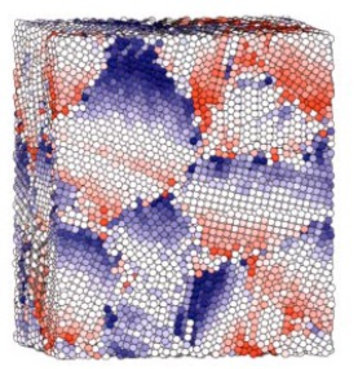
\includegraphics[width=0.3\textwidth]{figs/4-2_1.pdf}
  \caption{鉄の内部組織}
  \出典{○○○○(香山正憲(AIST))}
  \label{fig:2-2_sample}
\end{figure}

\rmproject{新量子相・新物質の基礎科学}
[ダミー原稿]、[ダミー原稿]、[ダミー原稿]、[ダミー原稿]、[ダミー原稿]、[ダミー原稿]、[ダミー原稿]、[ダミー原稿]、[ダミー原稿]。


\subsection{課題とその解決に必要な計算手法・アプリケーション}
計算物質科学で使われるアプリケーションは非常に多岐にわたる。
以下、計算物質科学分野における、現在の主要なアプリケーション・アルゴリズムの中から、凝縮系に対する第一原理計算、高精度分子軌道法、大規模分子軌道法、フラグメント分子軌道法、電子・電磁場ダイナミクス法、短距離力古典分子動力学法、長距離力分子動力学法、化学反応動力学法、量子分子動力学法、クラスターアルゴリズム量子モンテカルロ法、変分モンテカルロ法、厳密対角化、階層的マルチスケールシミュレーションについてとりあげ、その概略・特性と、今後5~10年で必要となる計算機スペックをまとめる。

\rmproject{第一原理計算(凝縮系)}
半導体材料、磁性材料、光学材料、金属材料などの固体材料を主な計算対象として発展してきた手法が密度汎関数理論(Density Functional Theory(DFT))に則った第一原理計算手法であり、第一原理分子動力学法やバンド計算法という名前で呼ばれることもある。
Kohn-Sham方程式(一電子シュレディンガー方程式)と、電荷密度分布が自己無撞着場(Self-consistent Field=SCF)を満たすように、波動関数と電荷密度分布を繰り返し更新することで解くこの手法の計算需要は、より大きな系の電子構造を精度よく求めるということの他に、長時間の分子動力学計算や統計的処理を行うことにより反応経路や自由エネルギー差などを評価するという、二つの方向に広がりつつある。
前者は大規模化を追求する方向性でweak scaling的である。後者にはstrong scalingを追求するものと、時間やレプリカなど別の軸に関する並列化により計算機能力の向上を有効利用しようとするものとがある。
また、励起状態、光学特性、電気伝導特性などの物性予測を高精度に行いたいという需要も大きい。

\subparagraphl{・O($N^3$)法}
扱う原子数$N$に対して演算量が$N^3$に比例する計算方法をO($N^3$)法、$N$に比例する計算方法をO($N$)法(オーダーN法)と呼ぶ。
伝統的なO($N^3$)法の場合、波動関数$\Psi$ を表現する$M$個の基底関数による$M$行$M$列のハミルトニアン行列を対角化して固有値を得るために$M^3$に比例する計算量が必要になるが、CarとParrinelloの提案した方法とそこから発展した方法では、SCFの繰り返しの中で反復解法を使ってより少ない演算数で固有値問題を解くことができる。基底関数の選び方には、結晶の周期性を利用した平面波を用いるもの、実空間格子点上の値を用いるものなどがある。全電子ではなく価電子だけを陽に扱う擬ポテンシャル法が大規模計算に適している。
価電子軌道の数を$B$とすると演算数は$B^2M$に比例する。典型的には、$B$は原子数$N$の数倍程度、$M$は100倍程度の値であり、O($N^3$)ではあるが$M^3$の演算数に比較すればずっと少ない。
ここでは擬ポテンシャル法第一原理計算の中で、平面波基底を用いるプログラムとして、PHASEとxTAPPを、実空間基底を用いるプログラムとしてRSDFTを挙げて解析する。
平面波基底は古典的基底でありFFTを頻繁に使うが、原子位置に対して計算精度が不変、行列要素を厳密に計算するのが容易である。
一方、実空間基底は、力の計算精度を上げるのに工夫がいるが、非局所ポテンシャルと波動関数の積の計算負荷が軽いこと、FFT演算を含まないことなどから大規模化に適しているとされる。
また周期境界条件に縛られないO($N$)法への展開が見込める。平面波基底を使う手法で大規模計算を行うためにはFFT演算にともなう通信を極力局所化する必要がある。
基底関数が何であれ、一回のSCFループ内の計算は、(i)グラムシュミット法などにより規格直交化する部分、(ii)波動関数を残差関数を使って更新する部分(残差最小化法(RMM)、共役勾配法(CG)、Block-Davidson法、最急下降法(SD)など)、(iii)部分対角化する(波動関数のユニタリー変換を行う)部分、(iv)波動関数から電荷密度分布をつくる部分、などからなる。

平面波基底の場合には、負荷の重い部分は、各種の行列・行列積O($B^2M$)と固有値問題O($B^3$)、FFT演算O($BM\log M$)などに分解することができる。
扱う原子数が多くなるに従いFFT演算部分の負荷は相対的に小さくなる。波動関数に関する3次元FFTはバンド(軌道関数)とFFTの1軸分あるいは2軸分を併せて分割することで、核心部のバタフライ演算はノード内(キャッシュ内)に閉じ込めて行い性能劣化を抑えることができる。
ただし、分割軸を交換するために局所的な転置転送通信を行う必要がある。
非局所ポテンシャルと波動関数の積はO($B^2M$)であるが、並列化効率の向上は容易である。
これに対し(iii)の部分対角化で使うO($B^3$)の固有値問題はそれが難しい。
大規模化するためにはこの部分の効率向上が必要であり、数値計算ライブラリの整備に期待する。
また、波動関数の規格直交化に用いるグラムシュミット法はスレッド並列版のBLASを用いて実装しているが、逐次実行部分が残っている。
これが並列化効率の制限因子の一つとなっている。
これに代わる手法の開発も必要である(TSQR法(AllReduce QR法)やCar-Parrinello法を改良した波動関数の規格直交化に用いるグラムシュミット法はスレッド並列版のBLASを用いて実装しているが、逐次実行部分が残っている。これが並列化効率の制限因子の一つとなっている)。

実空間基底を用いる方法は、FFT演算にともなう通信を局所化するなどの手間が要らない、非局所ポテンシャルと波動関数の積演算の負荷が軽いという違いはあるが、(i)規格直交化や(iii)部分対角化に関して抱える課題は、平面波基底を用いる方法と同じである。

O($N^3$)のアプリケーションは、うえで述べたように大規模化と、規模の拡大よりも動的性質を予測するといった方向性の両方を指向するが、ここではRSDFTでは10~100万原子規模の計算を目指し、平面波基底の手法は1万原子規模の系の動的性質を予測する方向を目指すものとして評価を行う。

\rmproject{高精度分子軌道法}
分子軌道法は、基本となるHartree-Fock法を出発点とし、摂動法、結合クラスター法、配置間相互作用法などにより電子相関を取り込み、計算精度を系統的に引き上げられるという特徴がある。
行列積、行列対角化、連立一次方程式計算、そして基底関数の軌道角運動量によって演算内容が異なる1電子・2電子積分計算が主な演算で、計算対象分子を分割しない限り、どの方法でも全対全通信を行う必要がある。
電子相関計算では、中間データ量が系の3乗もしくは4乗に比例して増加するため、各ノードに分散させてもノード当たりの必要メモリ量は多くなる。

エクサスケール計算機では、分光学的精度で分子構造や機能を予測することが期待される。
この目標は、露わに相関した結合クラスター法を完全基底関数極限で解くという、超高精度電子状態計算で達成される見込みである。
ここで、電子相関の計算で必要になる4中心2電子分子軌道積分を、3中心1電子分子軌道積分と求積点での分子軌道の値の積から数値求積法により計算する。
多電子積分計算についても同様に数値求積法で行う。
求積法で2電子積分を計算する部分と、それに続く計算部分をまとめることで演算量を減らすとともに、計算負荷およびデータ分散を容易にする。
主要な演算は行列-行列積である。各ノードに分散されている求積点ごとのデータを集めるため、通信はallreduce、gathervが大半である。以下、基底関数極限のフラーレン分子(2万基底、100万求積点)の計算、1ノード性能100TFLOPS、全体性能1EFLOPSを想定して見積もりを行う。

\subparagraph{【メモリ】}
2万×100万(160GB)の配列が4つ、更にその他の配列も考慮して1ノード当たり1Bが必要になる。
メモリバンド幅は、(2万×100万)×(2万×2万)の行列積演算では、1度だけメモリからデータが送られると仮定すると40GB/s、余裕を見て100GB/sが望まれる。
一連の操作を波動関数が収束するまで数十回繰り返し行う。

\subparagraph{【オンチップメモリ】}
求積法で計算する3中心1電子積分用として1GB程度は必要になる。

\subparagraph{【通信】}
2万×100万の配列をgathervで集めた後、上記の行列積演算を4回続けて行うので、計算時間の1割で受信を完了させるためにはノード当たり50GB/sのバンド幅が必要にな
る。

\subparagraph{【ストレージ】}
計算中のデータはすべてメモリに保存するため、出力するファイルは計算結果のみである。
そのサイズは100TB程度であり、0.01TB/sのファイルI/O性能が必要となる。

\rmproject{大規模分子軌道法}
Hartree-Fock法、密度汎関数法によるナノスケール分子の計算を行う。
大部分が2電子クーロン反発積分の計算であり、演算自体は複雑であるが比較的少量のデータを何度も利用するといった特徴がある。
Gauss関数の局所性を利用するため、IF文によるカットオフを多用している。
3次元ナノスケール分子(1万原子系、10万基底)計算を想定すると、30TFLOPSマシン1万ノードの場合、計算時間は1回当たり30分である。
安定構造を求めるためには、この計算を数十回繰り返す。

\subparagraph{【メモリ】}
10万×10万(80GB)の配列を、Fock行列、正準化変換、基底重なり、分子軌道、密度行列用に5つ用意するため、1ノード当たり400GB必要になる。
10万×10万の行列積をうため、密度汎関数計算での数値積分で1原子当たり1万点グリッドを発生させる場合、ノード当たりのFock行列へのアクセスデータ量は、10万×10万×1万(点数/原子)×1万(原子 / 1万(ノード)×8Byte = 800TBとなる。
カットオフによるデータ量削減(約10\%に削減)考慮し1分でこのアクセスを完了させるためには、ノード当たりのバンド幅は1.8TB/s必要になる。

\subparagraph{【オンチップメモリ】}
2電子積分計算のため、1コア当たり1MB必要となる。これは、(gg{\textbar}gg)型積分では、15×15×15×15のサイズの配列にデータを蓄え、同等程度の計配列も必要になるためである。

\subparagraph{【通信】}
計算1回(30分)あたり、80GB配列をallreduceで集める操作を30回程度行う。通信時間を全体の5\%にするには、バンド幅30GB/sが必要になる。

\subparagraph{【ストレージ】}
出力するファイルは計算結果のみで、そのサイズは100GB程度である。ファイルI/O性能は0.0001TB/s程度で十分である。

\rmproject{フラグメント分子軌道法}
フラグメント分子軌道(FMO)法は並列処理を駆使し、タンパク質の電子状態を量子論(QM)的に丸ごと計算することが可能な手法の一つである。
FMO計算は実際には、基本のHartree-Fockから高次相関法まで多種の近似がある。
一般に相関計算では、DGEMM等のBLASを使ったテンソル縮約が支配的で、軌道の添字を複数持つ多次元配列の操作となるためにB/Fが高いほうが性能的には有利である。
だたし、タイリングやブロッキング等を適宜導入することで0.1程度までは性能の保持が可能である。
メモリ要求値に関して述べれば、FMO2のダイマーでクラスター展開の計算では、作業配列の総容量はアミノ酸残基の組み合わせと基底関数にもよるが、数十GBには容易に達する。

現時点で、数百残基のタンパク質のPDB構造をベースにした一点でのFMO2計算はルーチン的に行えるようになってきているが、より実在的なモデリング手法として信頼性を高めるには、水和条件を課したうえで揺らぎを考慮するために分子動力学的に生成された多数の構造サンプルを扱った統計的な算定が望ましい。
また、3 体や4 体の展開(FMO3、FMO4)を行うことが、精度向上の観点から望ましい。フラグメントのトリマーやテトラマーの相対計算コストは数的には単純組み合わせよりは少ないが、個々のサイズが大型化するために増加する。2次摂動で数百残基のタンパクを扱う場合、FMO2に比してFMO3で3~5倍、FMO4では10倍程度である。サンプル数の設定によるが、FMO4で相関レベルを上げることまで考えれば、現行計算に比して要求される計算コストは数万~十万倍になるため、エクサ計算機で“統計的ジョブ”の高速実行が可能となれば、その科学的な恩恵はきわめて大くまた本質的なものとなる。

FMO計算は、光応答タンパク質の電子遷移エネルギーの定量的な算定でも使われてきている。
これは、応答部位(クロモフォア)を特定したうえで限定的に励起状態計算を行うものだが、エクサ級の超並列計算資源があれば、タンパク質全体について求めることも可能であろう。
物性値評価としても、2次高調波などの非線形光学応答核磁気共鳴などの磁気応答などもカバーされる。光合成系(PSC)の電荷分離のモデリングについても、FMO計算から得られるフラグメントMOを再構成する(FMO-LCMO)などの技法を用いて大域での電子移動度の算定が行えるようになると思われる。
そこでは数千万次元の非疎行列の固有値問題を解く必要がある。

計算機の環境について付言すると、米国のNWChemですでに活用されている多ノード共有メモリ空間構築と行列積ツール(GA)等が提供されると大規模フラグメントの処理には福音となると思われる。
また併せて、ノード間をまたぐスレッドベースの並列化もサポートされるとコードの発展には有利であろう。
“統計ジョブ”に関連しては、計算結果をダンする半導体メモリ(SSD)とともにフォルトトレランス機構が考慮されることが望まれる。

\rmproject{電子・電磁場ダイナミクス法}
光機能性を持った量子ナノ構造体デバイスを理論的に設計するための、電子・電磁場ダイナミクスの数値計算シミュレーションソフトウェアである。
対象とする系は、1辺十数nmから数十nm程度の実在系ナノ構造体。
原子数は100万原子から200万原子、時間ステップ数は2.5万~5万ステップである。

\subparagraph{【アルゴリズムの説明】}
時間依存Kohn-Sham方程式(方程式の形は時間依存シュレディンガー方程式と同一)を実空間3次元グリッド上で差分法を用いて解く。
x,y,z方向の格子点数を各々Nx,Ny,Nzとすると、実空間グリッドの総数はNx×Ny×Nzとなる。
主要な演算は、ハートリーポテンシャルを価するためのポアソン方程式の計算、時間発展計算にともなうハミルトニアンの波動関数への作用の二つに大別できる。
いずれにもラプラシアンの作用が含まれており、その演算は、((Nx×Ny×Nz)×(Nx×Ny×Nz))の疎行列と(Nx×Ny×Nz)のベクトルとの積と等価である。
ただし、実際の計算では疎行列そのものを扱うのではなく、縮約してベクトルとベクトルの積に帰着する。
マクスウェル方程式も実空間3次元グリッド上で差分法を用いて解くが、Kohn-Sham方程式に比べればその計算負荷は格段に低いので相対的に無視できる。

\subparagraph{【想定する計算】}
光機能性を持った量子ナノ構造体デバイスを設計するためには、最低50000ステップの時間発展が必要となる。
C60分子を立方体空間に25個×25個×25個~16000個並べる系を想定してスペックを見積もる。
この場合、原子数は60×16000分子~960000個軌道数は120×16000分子~1.9M軌道となる。

\subparagraph{【想定する計算機】}
時間発展1ステップ当たり1秒で計算を行うためには、630PFLOPSのシステムが必要になる。

\subparagraph{【計算空間総メッシュ数】}
メッシュサイズを0.25Åとすれば1辺当たり33nm÷0.25Å~1300。
したがって、総メッシュ数は(1300)3~2.2Gとなる。

\subparagraph{【総演算量】}
1ステップ当たり2.2G(総メッシュ数)×1.9M(総軌道数)×30回(差分法演算回)×5回(テーラー展開4次+軌道エネルギー評価)~630P回。

\subparagraph{【総メモリ量】}
計算グリッド上に波動関数をストアしておくためのメモリがほとんどを占める。
2.2G(総メッシュ数)×1.9M(総軌道数)×16B(複素数)×3(作用前波動関数用配列、後波動関数用配列、テーラー展開での総和の波動関数用配列)~200PB。

\subparagraph{【ネットワークバンド幅】}
1ステップ当たり2.2G(総メッシュ数)×8B(実数)~18GBの電子度用データのAllreduceによる通信が発生する。
通信を全実行時間の1割と考えるとノード当たり180GB/s必要となる。

\subparagraph{【メモリバンド幅】}
1ステップ当たりの総メモリ量を1秒でアクセスするために200PB/s必要となる。

\subparagraph{【オンチップメモリ】}
1軌道当たりに必要とされるメモリ量は2.2G(総メッシュ数)×16B(素数)×3(波動関数用配列数)~110GB。
空間を125分割(5×5×5分割)して、各ブロック内分法演算に使うデータをすべてオンチップ上に載せるためには0.9GB必要になる。

\subparagraph{【ストレージ容量】}
波動関数を入力として読み込むために、2.2G(総メッシュ数)×1.9M(軌道数)×8B(実数)~33PBが最低必要となる。

\clearpage
\subsection{ロードマップ}
\begin{figure}[H]
  \centering
  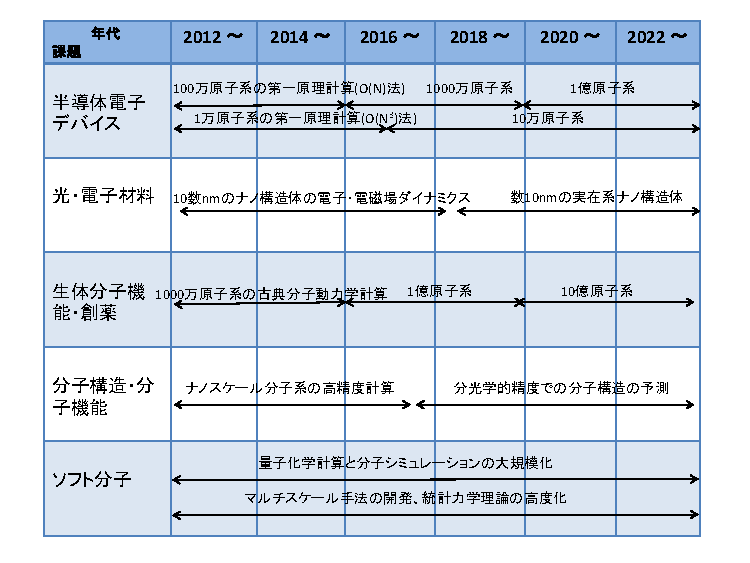
\includegraphics[width=0.7\textwidth]{figs/2-2_rm_1.pdf}
  \caption{物質科学ロードマップ(1)}
  \label{fig:roadmap_2-2_1}
\end{figure}
\begin{figure}[H]
  \centering
  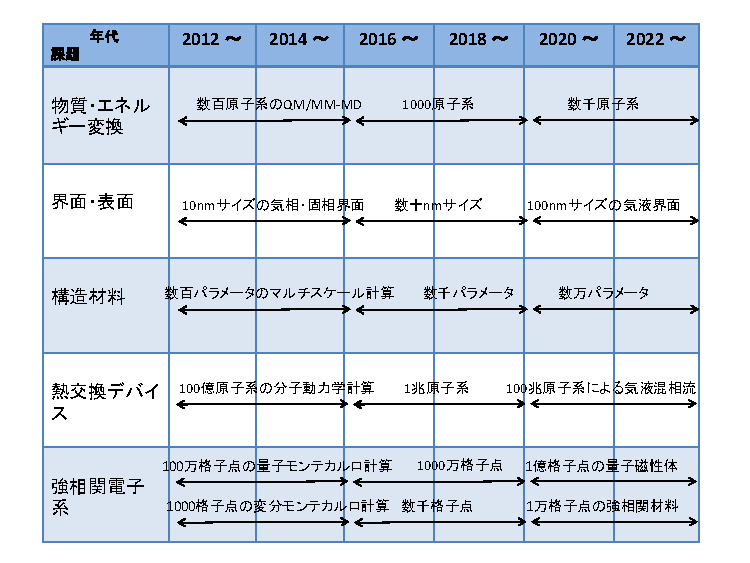
\includegraphics[width=0.7\textwidth]{figs/2-2_rm_2.pdf}
  \caption{物質科学ロードマップ(2)}
  \label{fig:roadmap_2-2_2}
\end{figure}

%\clearpage
\subsection{必要な計算機資源}
\input ReqSpecTabs/2-2.tex

% 参考文献
\nocite{*}
\bibliographystyle{\rmbibstyle}
\bibliography{2-2}
